\subsection{Diffraction in Crystals} \label{chap2}

\subsubsection*{Geometric Structure Factor} 

The structure factor gives the amplitude of a scattered wave arising
from the atoms with a single primitive cell. 
\begin{equation}
\mathrm{\Phi_k} = \sum_{j} f_j(\mathrm{K)}e^{i\mathrm{K \cdot d}}
\end{equation}
For crystals composed of only one type of atom, it’s common to split
the structure factor into two parts:
\begin{equation}
\mathrm{\Phi_k} = f_j\mathrm(K)S_{\mathrm{K}}
\end{equation}
,where $f_j$ is atomic form factor and $S_\mathrm{K}$ is geometric structure factor. Now let's focus on the second one.
\begin{equation}
S_\mathrm{K} = \sum_{j = 1}^{n} e^{i \mathrm{Kd}}
\end{equation}

For a perfect crystal the lattice gives the reciprocal lattice, which determines the positions (angles) of diffracted beams, and the basis gives the structure factor $F_{hkl}$ which determines the amplitude and phase of the diffracted beams:
\begin{equation}
F_{hkl} = \sum_{j = 1}^{N} f_j \mathrm{e}^{[-2\pi i(hx_j + ky_j + lz_j)]}
\end{equation}

As seen in \autoref{chap1} a FCC unit cell contains 4 atoms, one at the origin $ x_j, y_j, z_j = (0, 0, 0)$ and one at the three adjacent face centers $ x_j, y_j, z_j = \Big(\frac{1}{2}, \frac{1}{2} , 0\Big), \Big(0, \frac{1}{2} , \frac{1}{2}\Big)\ \mathrm{and}\  \Big(\frac{1}{2} , 0 , \frac{1}{2}\Big) $

$$
F_{hkl} = \sum_{j = 1}^{4} f_j \mathrm{e}^{[-2\pi i(hx_j + ky_j + lz_j)]} = f[1 + (-1)^{h+k} + (-1)^{k+l} + (-1)^{h+l}]
$$

with the result

$$
F_{hkl} = 
\left\{ \begin{array}{ll}
4f, & h,k,l\ $all even or all odd$ \\
0, & h,k,l\ $mixed parity$\\
\end{array} \right.
$$

\begin{itemize}
\item lattice centering (translational operations derived from the lattice type)
\item screw axes (symmetry axes that imply rotation and an additional translation)
\item glide planes (mirror planes that imply reflection and an additional translation).
\end{itemize}


\subsubsection*{Diffraction Maximums}
Bragg diffraction occurs when radiation, with a wavelength comparable to atomic 
spacings, is scattered in a specular fashion by the atoms of a crystalline system, and 
undergoes constructive interference. For a crystalline solid, the waves are scattered 
from lattice planes separated by the interplanar distance $d$. Bragg's law,  describes 
the condition on for the constructive interference to be at its strongest by formula:
\begin{equation}
\label{Bragg}
2d_{hkl} \sin{\theta} =  \lambda
\end{equation}
We need to use the concept of the reciprocal lattice to evaluate the lattice structure
factor $S$, which is involved in the x-ray scattering process. In equation:
\begin{equation}
S = G_{hkl}
\end{equation}
The scattering vector s is equal to a
reciprocal lattice vector.Also this implies that $s$ is normal to the $(hkl)$ crystal planes. For a cubic system we gave also a formula:
\begin{equation}
\frac{1}{d^2} = \frac{h^2 + k^2 + l^2}{a^2}
\end{equation}
After few transformation we get:
$$
d_{hkl} = \frac{a}{\sqrt{h^2 + l^2 + k^2}}
$$

Planes where we obtain a first 3 difraction maximums are following: 
(These are the first three planes which meet the condition of all
indices even or all odd)

$$P_1 = (111) \qquad P_2 = (200) \qquad P_3 = ( 220) $$ 

We can calculate interplanar distances:

$$d_{111} = \frac{5,58}{\sqrt{1^2 + 1^2 + 1^2}} = 3,23 \AA$$
$$d_{200} = \frac{5,58}{\sqrt{2^2 + 0^2 + 0^2}} = 2,79 \AA$$
$$d_{220} = \frac{5,58}{\sqrt{2^2 + 2^2 + 0^2}} = 1,98 \AA$$

Now we can calculate the Bragg angles for the corresponding maximas.
For the X-Ray wavelength $\lambda = 1.54 \, \mathring{A}$

$$
sin \theta = \frac{\lambda}{2d}
$$
$$
\theta = \arcsin{\frac{2d}{\lambda}}
$$

$$
\theta_1 = 13,3^\circ \qquad \theta_2 = 15,7^\circ \qquad \theta_3 = 22,3^\circ
$$


\subsubsection*{Reciprocal Lattice}
In order to identify the reciprocal lattice we start by the calculating
the reciprocal lattice vectors, which form a new set of basis vectors.

As in \autoref{chap1} already explained the three primitive vectors
of the FCC structure are:

$$\vec{u} = \frac{a}{2} \left(\begin{matrix}1\\1\\0\\\end{matrix}\right) \qquad
\vec{v} = \frac{a}{2} \left(\begin{matrix}0\\1\\1\\\end{matrix}\right) \qquad
\vec{w} = \frac{a}{2} \left(\begin{matrix}1\\0\\1\\\end{matrix}\right)$$

The new reciprocal lattice vectors are defined as:

\begin{equation}
    \vec{u^*} = \frac{2 \pi}{V_{PC}} (\vec{v} \times \vec{w}) \qquad
    \vec{v^*} = \frac{2 \pi}{V_{PC}} (\vec{w} \times \vec{u}) \qquad
    \vec{w^*} = \frac{2 \pi}{V_{PC}} (\vec{u} \times \vec{v})
\end{equation}

With $V_{PC}$ the volume of the primitive cell given from \autoref{chap1}
as:
$$V_{PC} = \frac{a^3}{4}$$

The three vectors result in:

$$
    \vec{u^*} = \frac{2\pi}{a} \left(\begin{matrix}1\\1\\-1\\\end{matrix}\right) \qquad
    \vec{v^*} = \frac{2\pi}{a} \left(\begin{matrix}-1\\1\\1\\\end{matrix}\right) \qquad
    \vec{w^*} = \frac{2\pi}{a} \left(\begin{matrix}1\\-1\\1\\\end{matrix}\right)
$$

Which represents the primitive translation vectors of a BCC lattice.
Therefore the bcc lattice is the reciprocal lattice to the FCC lattice
in which calcium crystallizes.


\subsubsection*{Edwald Sphere}

If we draw the wavevector $\mathbf{k}$ in the reciprocal lattice and let it
terminate at any reciprocal lattice point.
We draw a sphere of the radius $k=2\pi/ \lambda$ about the origin of $\mathbf{k}$
A diffracted beam will be formed if this sphere intersects any other point in the 
reciprocal lattice.
The $\mathbf{G_{\overline{2}\overline{1}0}}$ vector represent the 
$(\overline{2}\overline{1}0)$ plane.

\begin{figure}[H]
	\centering
	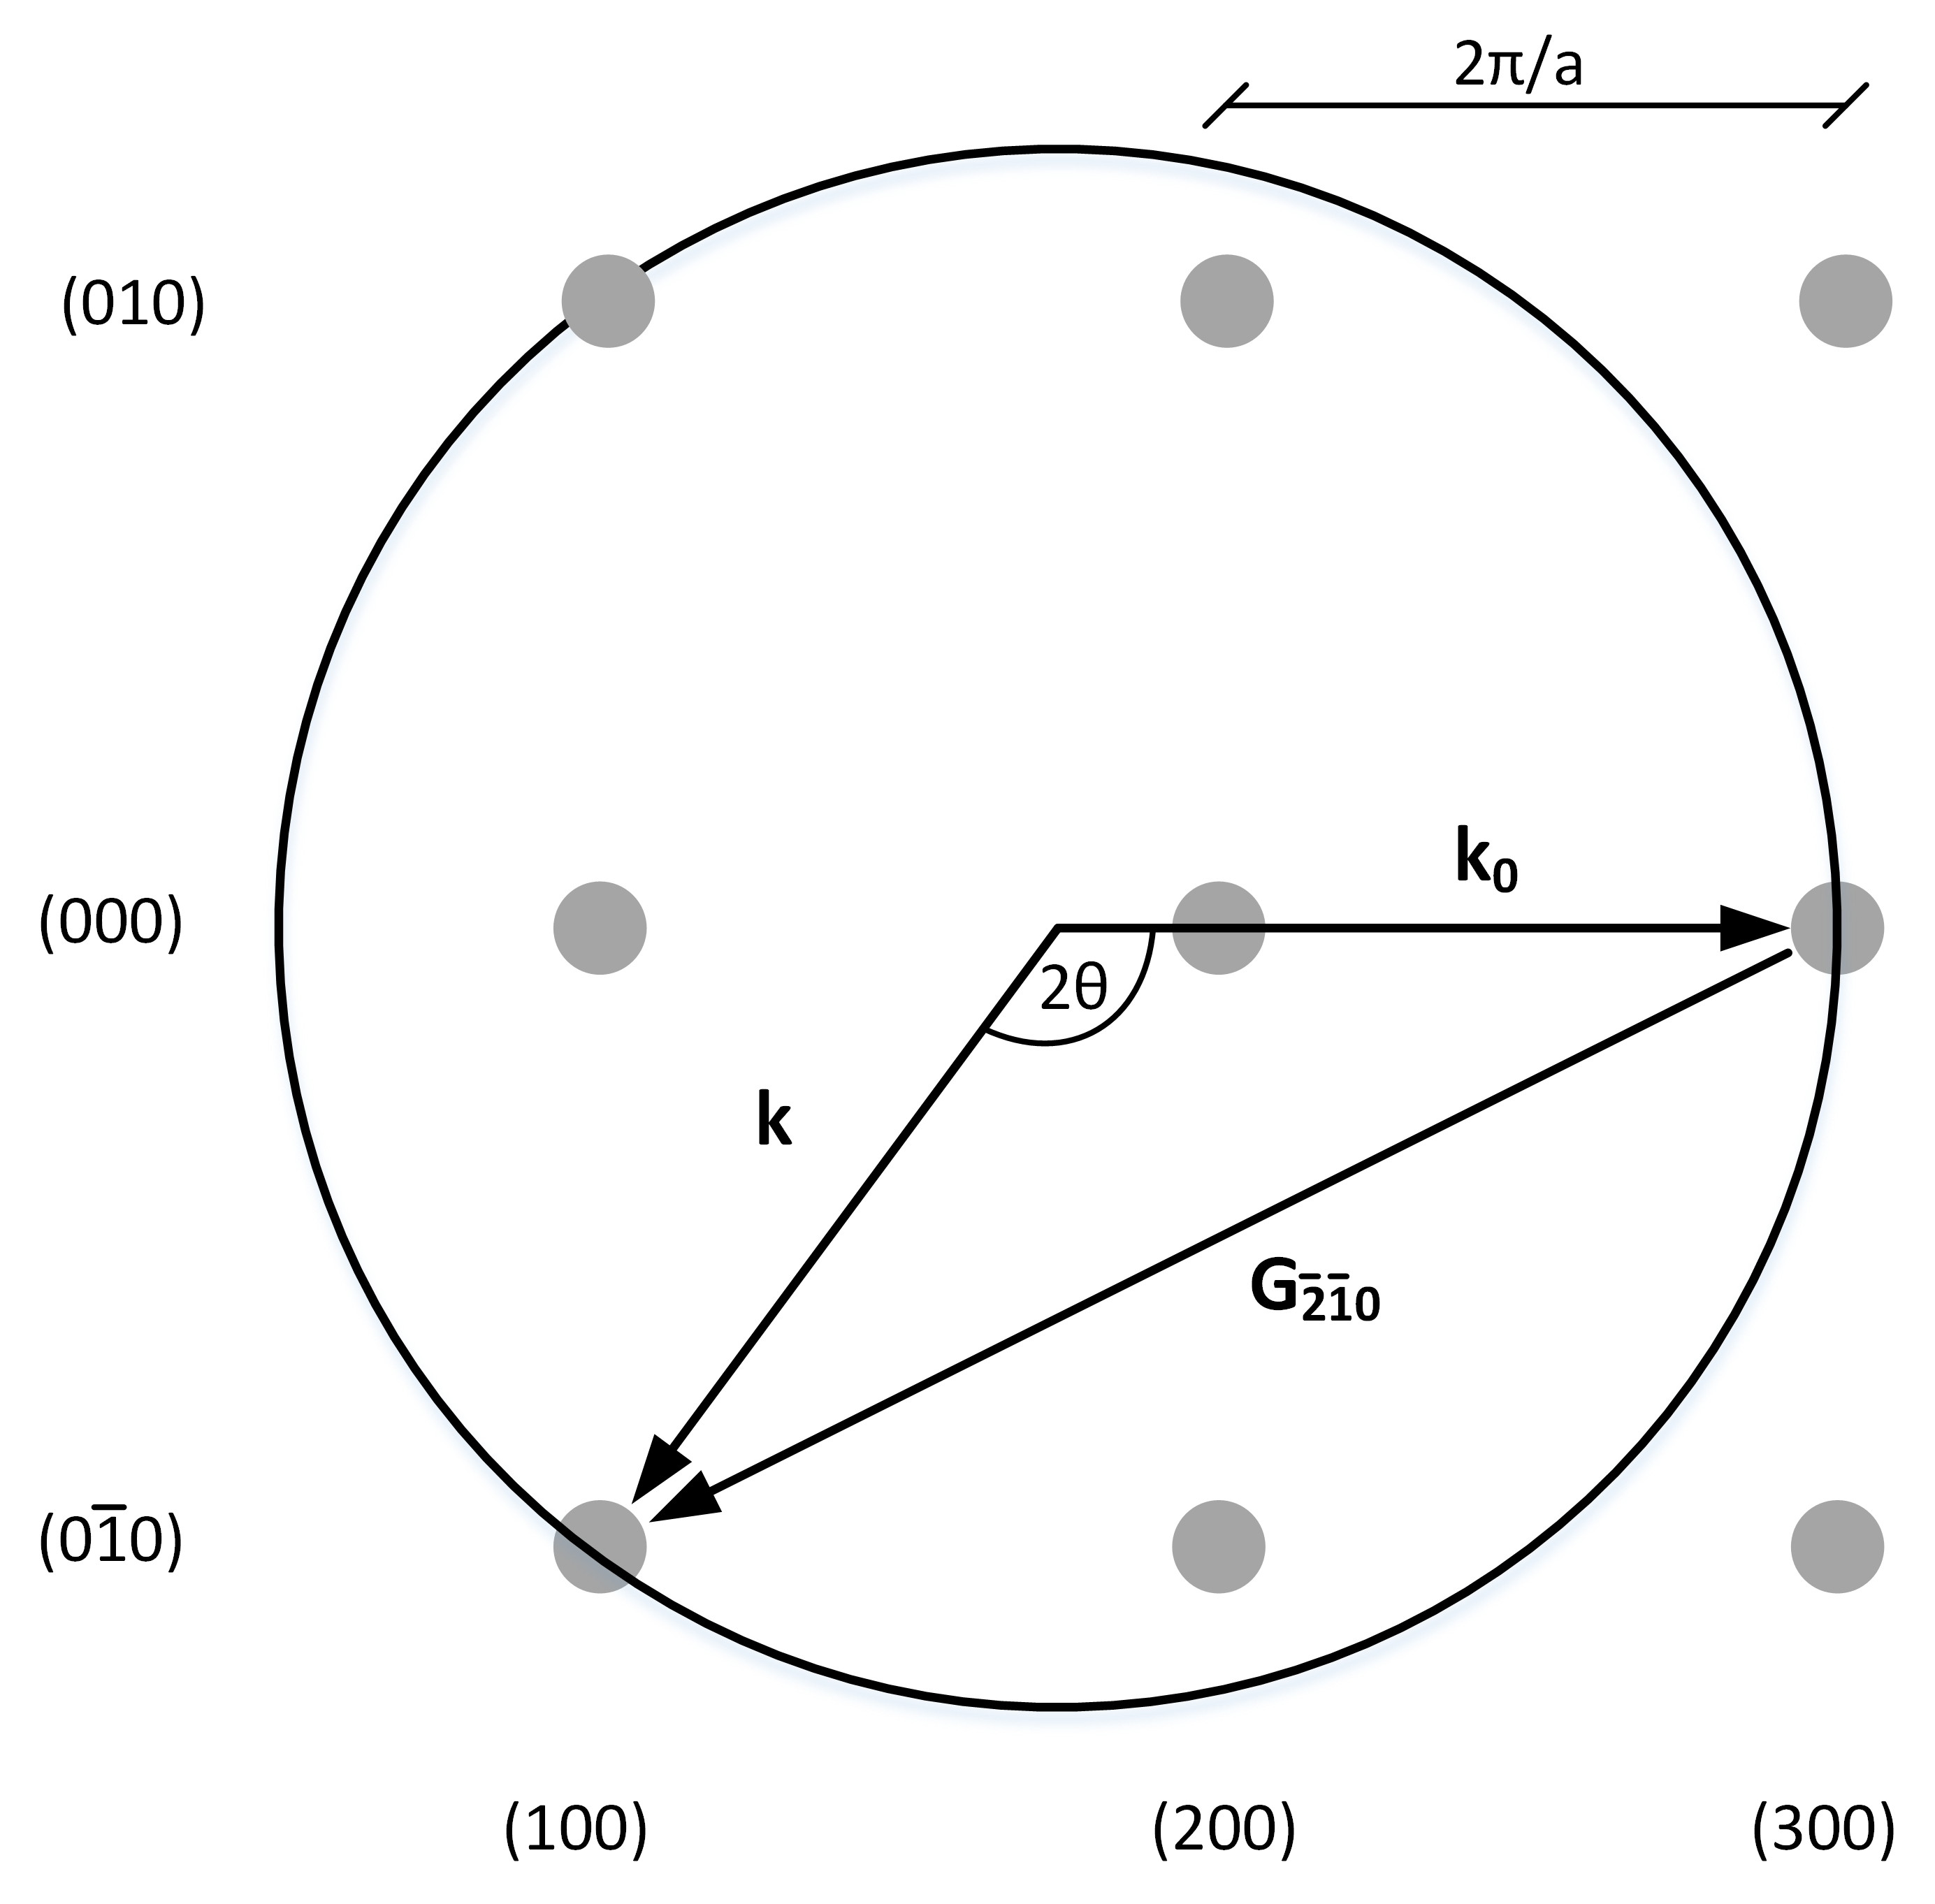
\includegraphics[width=0.5\linewidth]{Graphics/Chapter2/ewald_sphere.png}
	\caption{Ewald Sphere}
	\label{fig:ewals_sphere}
\end{figure}

Due Geometric to considerations the following relation can be derived.

$$\frac{G_{\overline{2}\overline{1}0}}{2a^*} = \frac{2 k_0}{G_{\overline{2}\overline{1}0}} \qquad \Rightarrow k_0 = \frac{5a^*}{4} = \frac{5\pi}{2a}$$

As for the wavelength $\lambda$  (with $a = 5.56 \, \mathring{A}$):

$$\lambda = \frac{2\pi}{k_0} = \frac{4a}{5} = 4.45  \, \mathring{A}$$

As for the angle $2\theta$ follows

$$2\theta = 180^\circ - 2 \cos^{-1} \left( \frac{G_{\overline{2}\overline{1}0}}{2k_0} \right) =
    180^\circ - 2 \cos^{-1} \left( \frac{\sqrt{5}}{10} \right) = 25.84 ^\circ$$